
%(BEGIN_QUESTION)
% Copyright 2009, Tony R. Kuphaldt, released under the Creative Commons Attribution License (v 1.0)
% This means you may do almost anything with this work of mine, so long as you give me proper credit

How much air pressure will be required to compress this valve actuator spring three-quarters of an inch, assuming it begins in a relaxed state with no air pressure applied?  Assume a $k$ value for the spring of 1340 lb/in, and a diaphragm diameter of 14 inches.

$$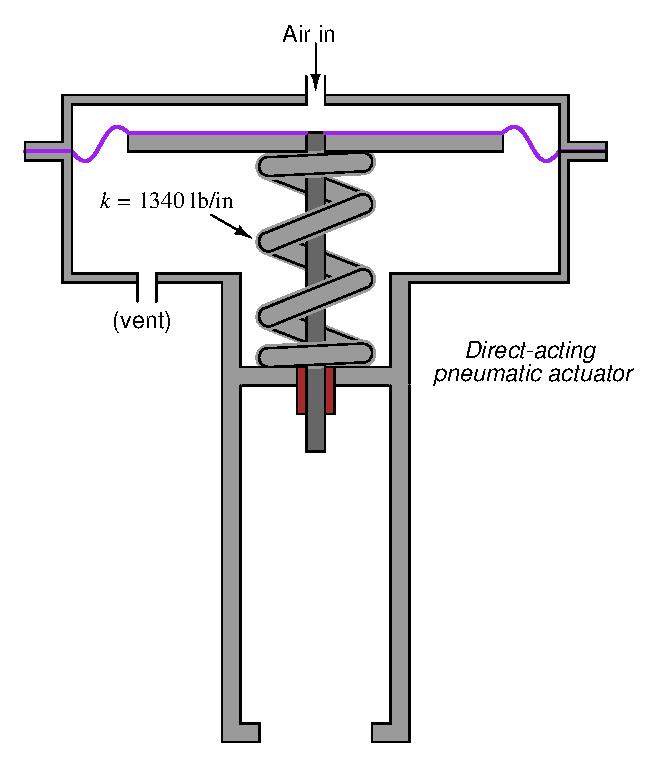
\includegraphics[width=15.5cm]{i03780x01.eps}$$

\underbar{file i03780}
%(END_QUESTION)





%(BEGIN_ANSWER)

The necessary compression force is 1005 pounds (1340 lb/in $\times$ 0.75 in).  With a diaphragm area of 153.9 square inches, this yields a pressure of 6.53 pounds per square inch.

%(END_ANSWER)





%(BEGIN_NOTES)


%INDEX% Physics, fluids: pressure, force, and area

%(END_NOTES)


